\chapter{The Compact Muon Solenoid (CMS) Experiment}

The CMS Experiment is a multipurpose particle detector located on the LHC ring underneath the Franco-Swiss border at CERN in Geneva, Switzerland. An overview of the experiments on the LHC ring can be seen in Figure~\ref{fig:LHCRing}. The experiment is located 100 meters underground in Cessy, France. CMS is 28.7 meters long, 15.0 meters in diameter, and weighs approximately 14,000 tonnes. It's arranged in a cylindrical, multi-layered structure consisting of a "barrel" and two endcaps, with the LHC beam passing through the vertical axis of the cylinder. CMS consists of several subdetectors, each designed to measure a different class or property of particle. From the beam line outward, the layers of CMS are the tracker, the electromagnetic calorimeter (ECAL), the hadronic calorimeter (HCAL), the superconducting solenoid, and the muon system (interspersed with the steel return yoke). A photograph of CMS can be seen in Figure~\ref{fig:CMSphoto}.

\begin{figure}\centering
  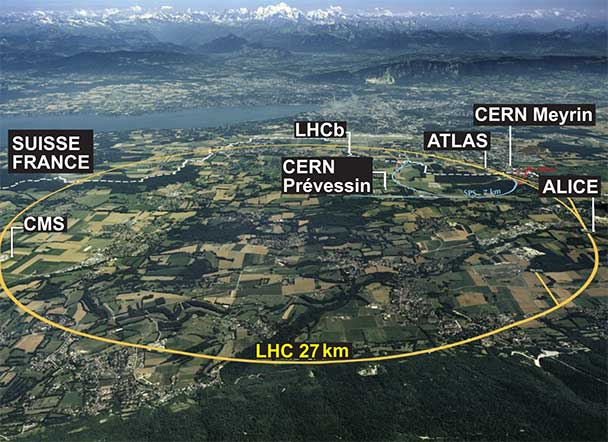
\includegraphics[width=0.4\textwidth]{figures/LHCRing.jpg}
  \caption{\label{fig:LHCRing} The Large Hadron Collider located underneath the Franco-Swiss border at CERN near Geneva, Switzerland. The CMS Experiment is located on the French side in Cessy, France}
\end{figure}

\begin{figure}\centering
  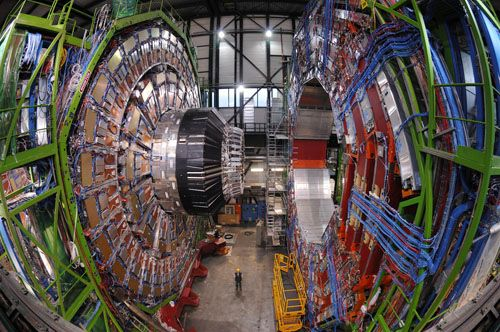
\includegraphics[width=0.4\textwidth]{figures/CMSphoto.jpg}
  \caption{\label{fig:CMSphoto} The CMS Experiment (open for maintenance)}
\end{figure}


The experiment uses a right-handed coordinate system: the origin is set at the $pp$ collision point, with the $x$-axis pointing towards the center of the LHC ring, the $y$-axis pointing straight up, and the $z$-axis pointing along the beam line in the counter-clockwise direction. CMS also uses a pseudo-polar coordinate system, with $\theta$ defined as the polar angle from the beam axis, and $\eta$ as the "pseudorapidity", itself defined as 


\begin{equation} \centering
$$
$ \eta = -ln\left[tan\left(\theta/2\right)\right] $
 $$
 \end{equation}

A diagram highlighting the layout of CMS can be seen in Figure~\ref{fig:CMSdiagram}.

\begin{figure}\centering
  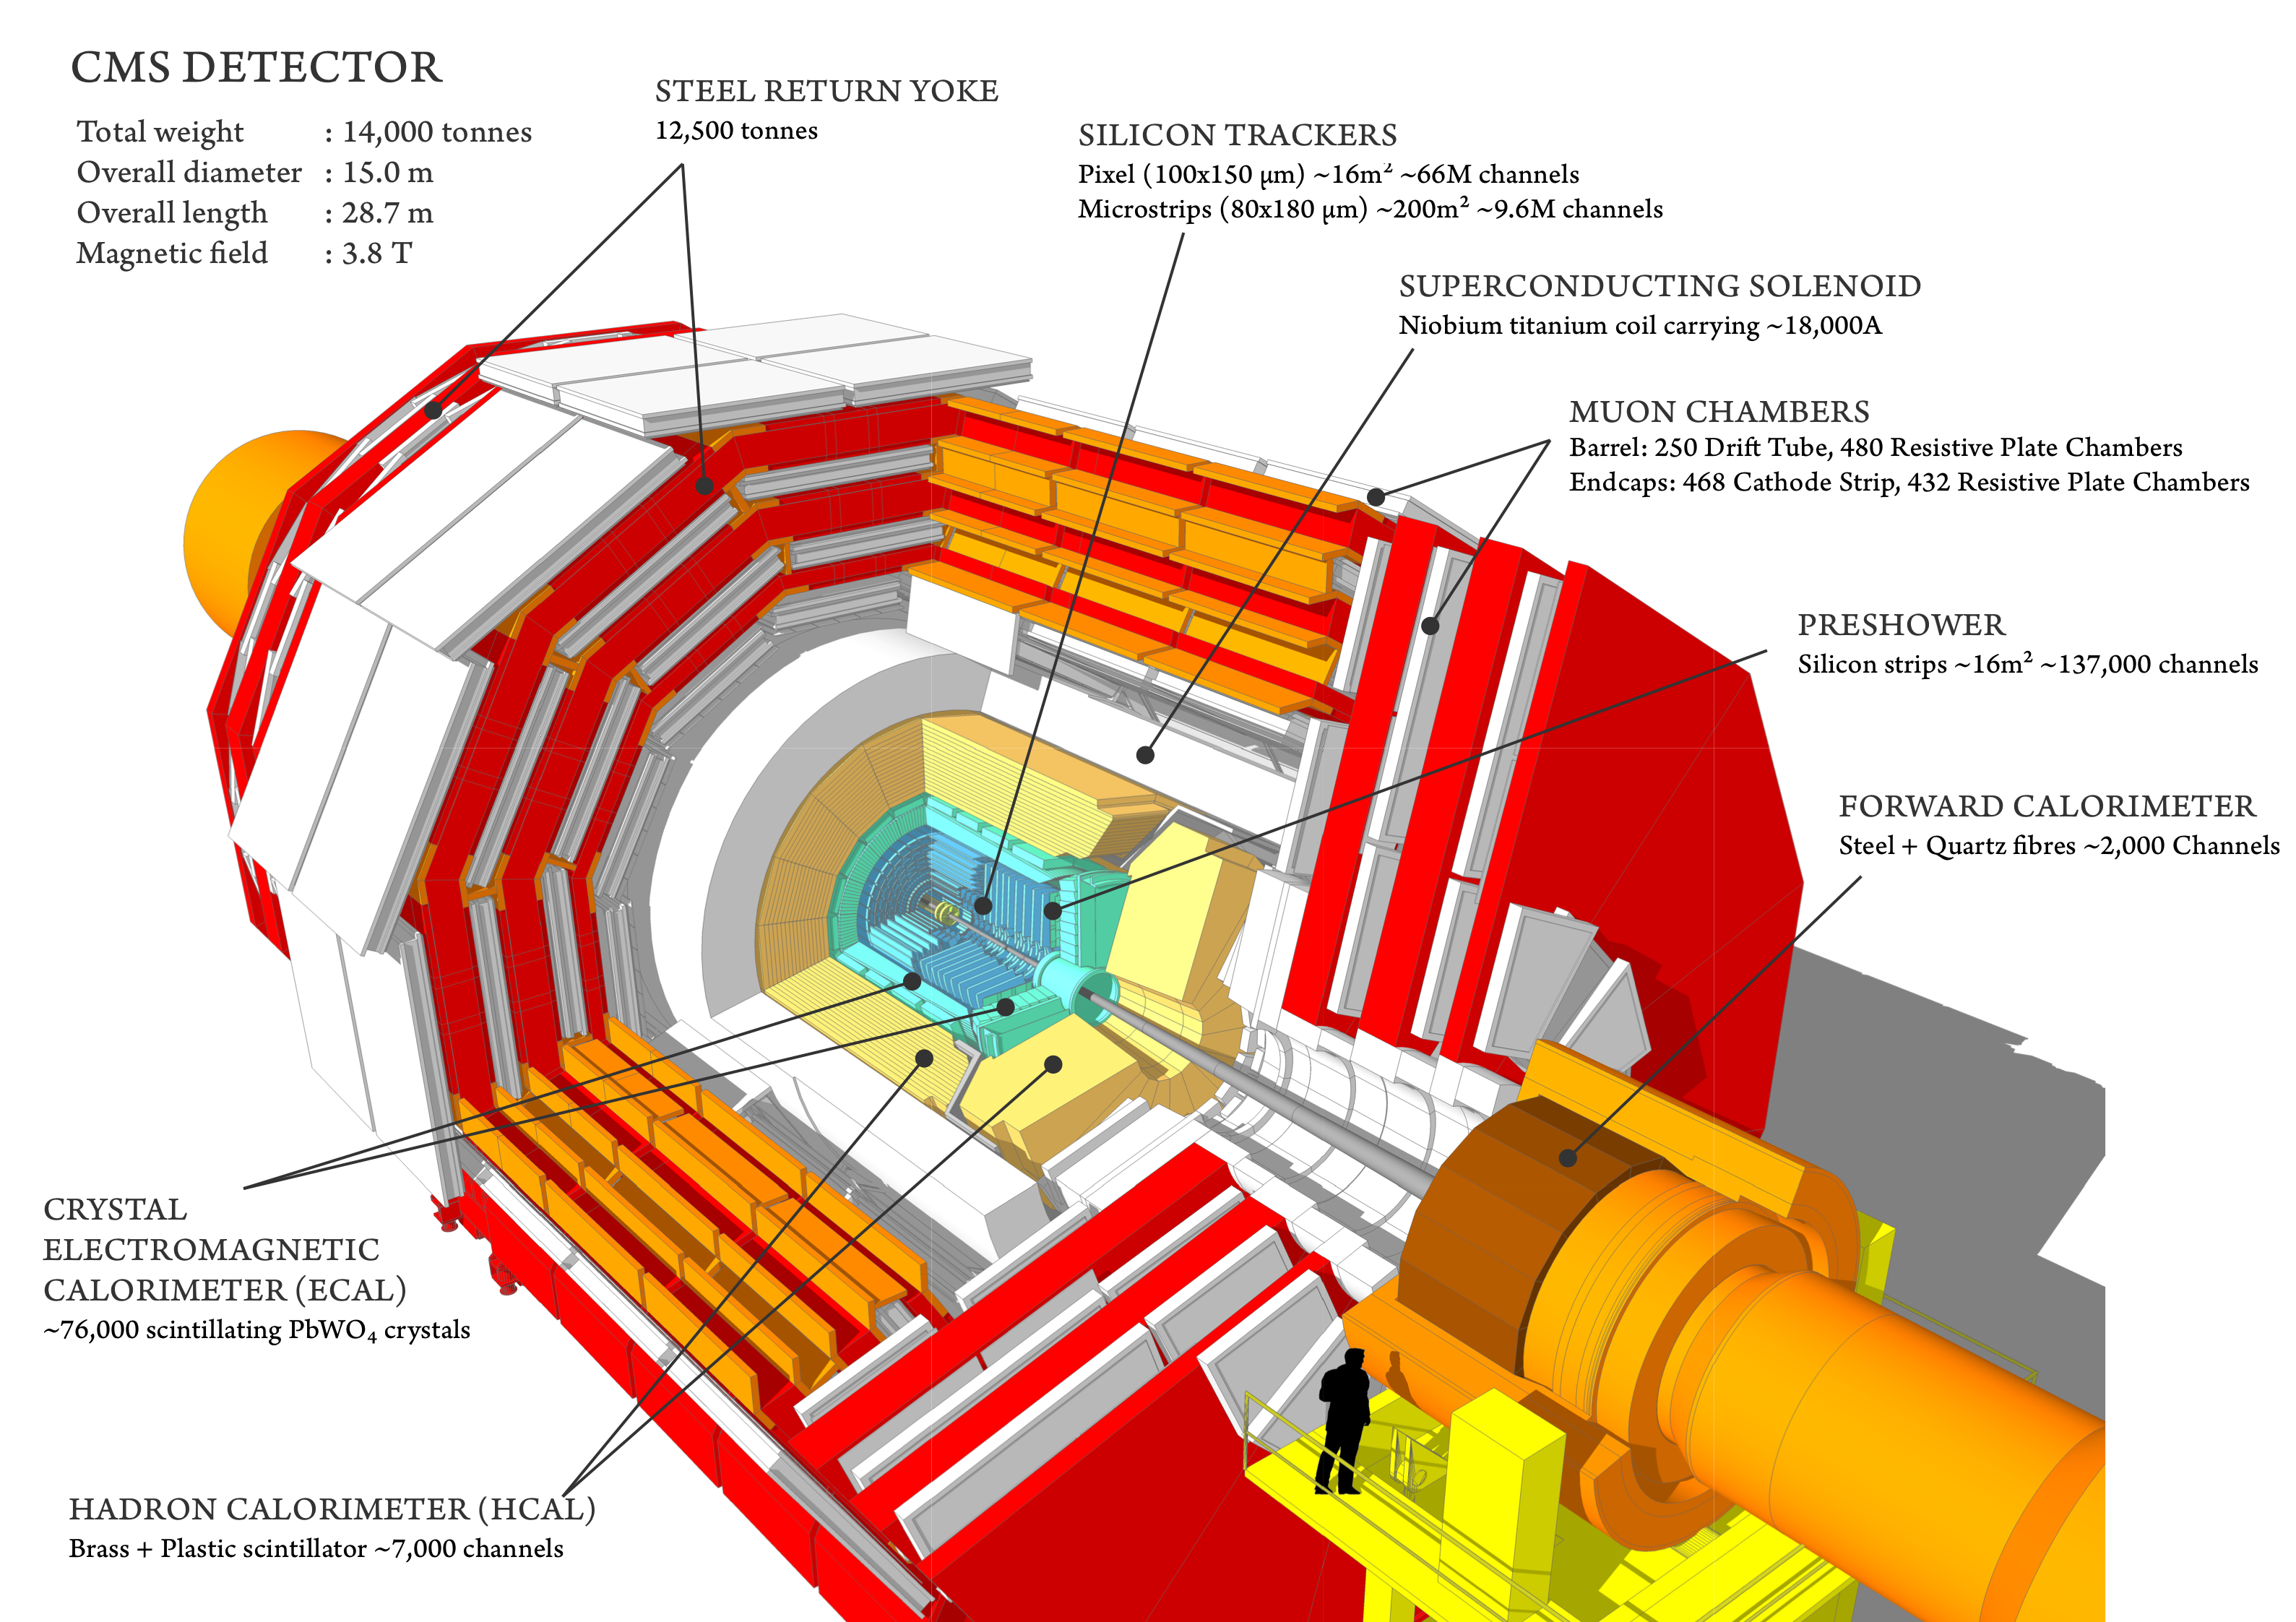
\includegraphics[width=0.4\textwidth]{figures/CMSdiagram.png}
  \caption{\label{fig:CMSdiagram} Schematic of the CMS Experiment showing the silicon trackers, electromagnetic calorimeter (ECAL), hadronic calorimeter (HCAL), superconducting solenoid, steel return yoke, and muon system.}
\end{figure}

\section{The silicon tracker}

The silicon tracker is the innermost detector element in CMS, and is designed to offer the highest resolution measurement of charged particle trajectories (such trajectories are referred to as ``tracks"). The tracker is composed of approximately 200m$^{2}$ of silicon, and includes arrays of silicon pixels in the inner layer and arrays of silicon strips in the outer layer. The silicon elements are arranged in the densest configuration near to the interaction vertex ($ r\approx 10$cm), with pixel size $\approx 100$ x $150 \mu$m$^{2}$. As one moves away from the interaction vertex, the solid angle becomes large enough that the particle flux drops off to a degree that larger silicon elements may be used (silicon strips measuring 10cm x 80$\mu$m at $20$cm$ < r < 55$cm, silicon strips measuring 25cm x 180$\mu$m for $r > 55$cm. The total number of silicon elements is 66 million pixels and 9.6 million strips. The tracker is divided into a barrel segment and two forward endcaps. The endcaps contain two pixel and nine strip layers each, and the barrel segment is separated into an inner and outer barrel. A schematic of the tracker layout can be seen in Figure~\ref{fig:TrackerLayout}. Particle tracks are reconstructed from hits in the individual silicon pixels/strips, the track being interpolated between hits.

\begin{figure}\centering
  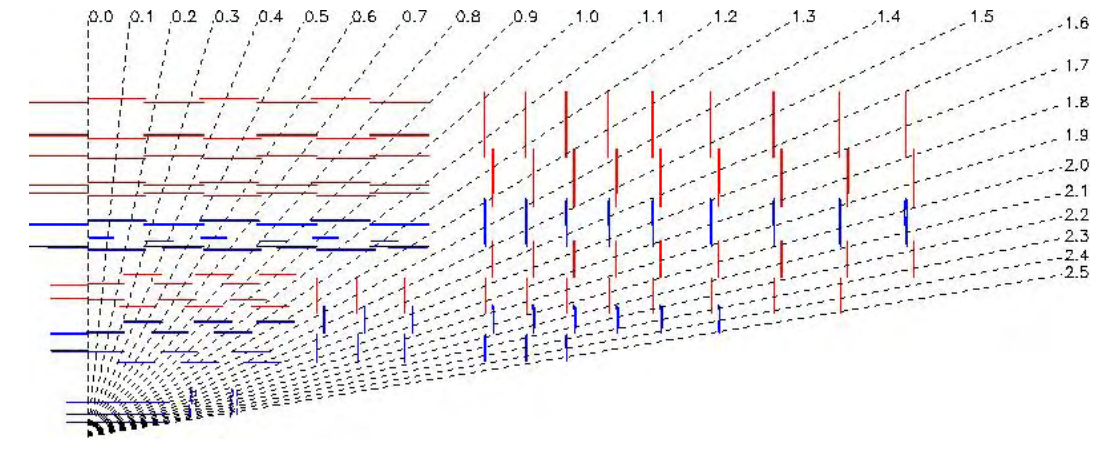
\includegraphics[width=0.4\textwidth]{figures/TrackerLayout.png}
  \caption{\label{fig:TrackerLayout} Overview of the silicon tracker layout.}
\end{figure}


\subsection{The pixel detector}

The pixel detector, shown in Figure ~fig(PixelLayout), consists of three barrel layers and two endcap layers. The barrel has a length of 53 cm, and the endcap disks range from 6 cm to 15 cm in radius. The pixel modules are arranged in a ladder-like configuration in the barrel, with 768 total modules comprising the barrel. The endcap disks are arranged in a turbine-like fashion, with 24 "blades" per disk, and 7 pixel modules per blade for a total of 672 pixel modules in the endcaps.
Each pixel consists of a readout chip (ROC), which are bump bonded to the modules. In total, the pixel detector includes about 16,000 ROCs.

\begin{figure}\centering
  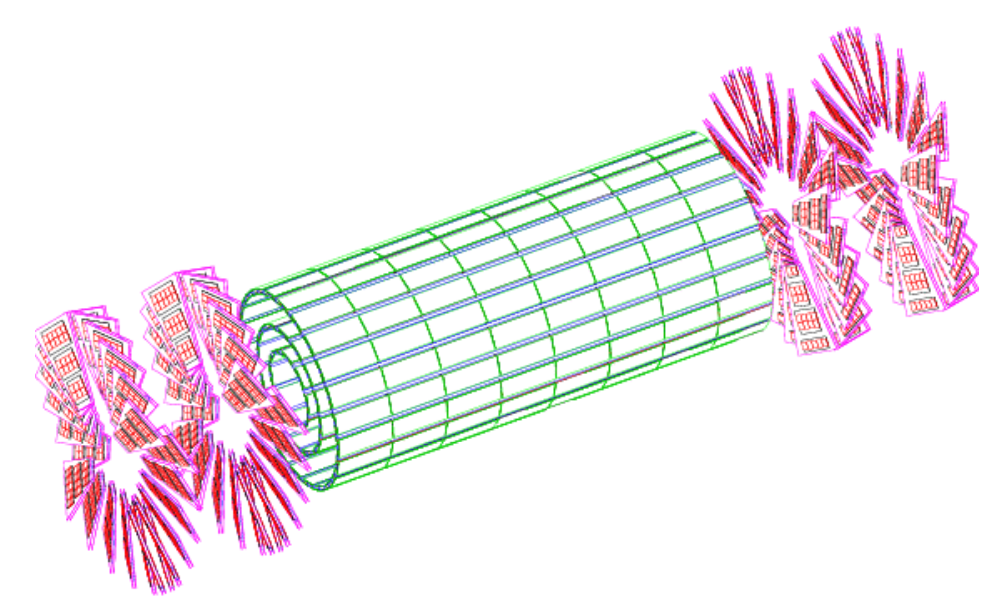
\includegraphics[width=0.4\textwidth]{figures/PixelLayout.png}
  \caption{\label{fig:PixelLayout} Diagram indicating the layout of the barrel pixel (BPIX) sensors (in green) and endcap pixel (FPIX) sensors (in pink)}
\end{figure}

\subsection{The strip tracker}

The strip tracker is divided into a barrel segment and two endcap segments. The barrel segment is itself divided into a Tracker Inner Barrel (TIB) section and a Tracker Outer Barrel (TOB) section. The TIB includes four layers of silicon strips each 320$\mu$m thick and ranging in pitch from 80$\mu$m and 120 $\mu$m. In the TOB, the lower rate of particle flux allows for larger strips (each 500$\mu$m thick and ranging in pitch from 120$\mu$m to 180$\mu$m).

The endcaps are each comprised of a Tracker Endcap (TEC) and Tracker Inner Disks (TIDs). The TIDs are designed to fill the region between the TEC and the TIB. The TECs each contain nine disks, and each TID contains three disks. On each disk, the modules (for both TID and TEC) are arranged in rings centered on the beam line. The TID strips (and three innermost ring strips of the TEC) have thickness 320$\mu$m, while the rest of the TEC strips have thickness 500$\mu$m. In total the strip tracker contains about 15,400 strip modules.  



\section{The electromagnetic calorimeter}

The next layer outward from the silicon tracker is the electromagnetic calorimeter (ECAL), which is designed primarily to measure energies of photons and electrons. The ECAL consists of an array of about 75,000 lead tungstate (PbWO$_4$) crystals, and has a barrel (BE) segment as well as two endcap (EE) segments. The BE segment has 61,200 crystals, while each EE segment contains 7,324 crystals.

PbWO$_4$ was chosen for the ECAL due to its short radiation length ($X_0 = 0.89$ cm), fast response time ($80\%$ of light emitted within 25ns), and radiation hardness (up to 10 Mrad).

The barrel (EB) crystals present an apparent cross-section (when viewed from the interaction vertex) of $\approx 22$x$22$ mm$^2$, and are 230 mm (25.8 radiation lengths) thick. The barrel has an inner radius of 129 cm, and covers the pseudorapidity range $0 < |\eta| < 1.479$.

The endcap (EE) crystals are each arranged in two D-shaped semicircular aluminum plates. From these plates are cantilevered "supercrystal" structures consisting of 5x5 crystal blocks. Each crystal presents an apparent cross-section of $\approx 28.6$x$28.6$ mm$^2$, and are 220 mm (24.7 radiation lengths) thick, and the endcap crystals cover the pseudorapidity range $1.479 < |\eta| < 3.0$.

A diagram of the ECAL layout can be seen in Figure~\ref{fig:ECAL_layout}.

\begin{figure}\centering
  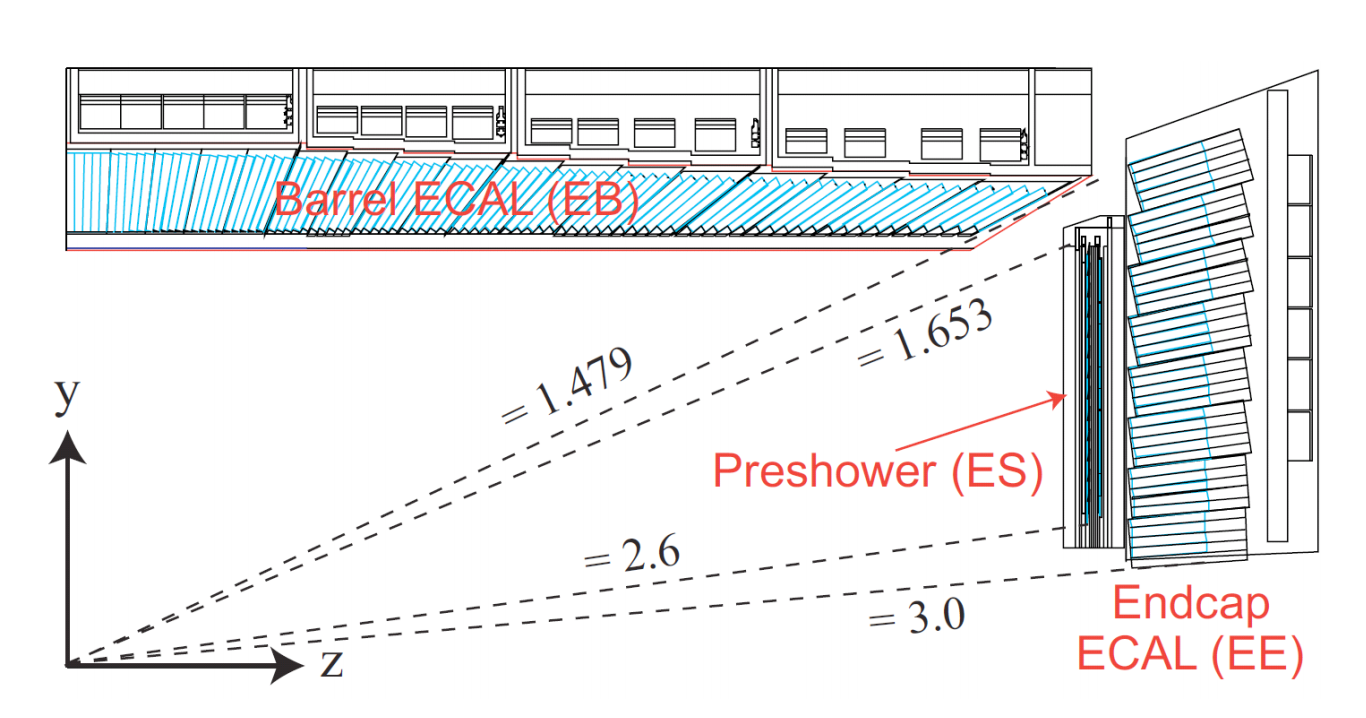
\includegraphics[width=0.4\textwidth]{figures/ECAL_layout.png}
  \caption{\label{fig:ECAL_layout} Layout of the electromagnetic calorimeter (ECAL) indicating the configuration of the barrel (EB) and endcap (EE) crystals.}
\end{figure}


\section{The hadronic calorimeter}

Surrounding the ECAL is the hadronic calorimeter (HCAL). The primary function of the HCAL is to measure the energies of hadrons (particles made of quarks and gluons). Located just inside the solenoid magnet, the HCAL is primarily composed of brass panels made from melted-down artillery shells. Interspersed with the brass panels are plastic scintillation panels, in which are embedded wavelength-shifting (WLS) fibers, which carry the signal to clear fibers outside the scintillators for readout. As hadrons enter the HCAL, they produce secondary particles in the brass which in turn create further particles. These hadron "showers" then interact with the plastic scintillators, where the fibers carry the signal to hybrid photodiodes so the signal can be measured.

HCAL is divided into barrel (HB) and endcap (HE) portions. Due to limited space between the ECAL and solenoid, the HCAL also includes material outside the solenoid: the outer HCAL (HO) lining the solenoid, and the forward calorimeter (HF) outside the muon endcap system. These additions increase the total radiation lengths covered by the HCAL to 10.

While HB and HE use the brass-plastic configuration, HO uses the solenoid itself instead of the brass, although the same plastic scintillators are used. The HF uses steel in place of brass, and quartz fibers in place of plastic scintillators. This is done to preferentially select neutral components of hadron showers, which are shorter and narrower and are thus well suited for the forward environment, which tends to be quite congested with particles.

A diagram of the HCAL layout is shown in Figure~\ref{fig:HCAL_layout}.

\begin{figure}\centering
  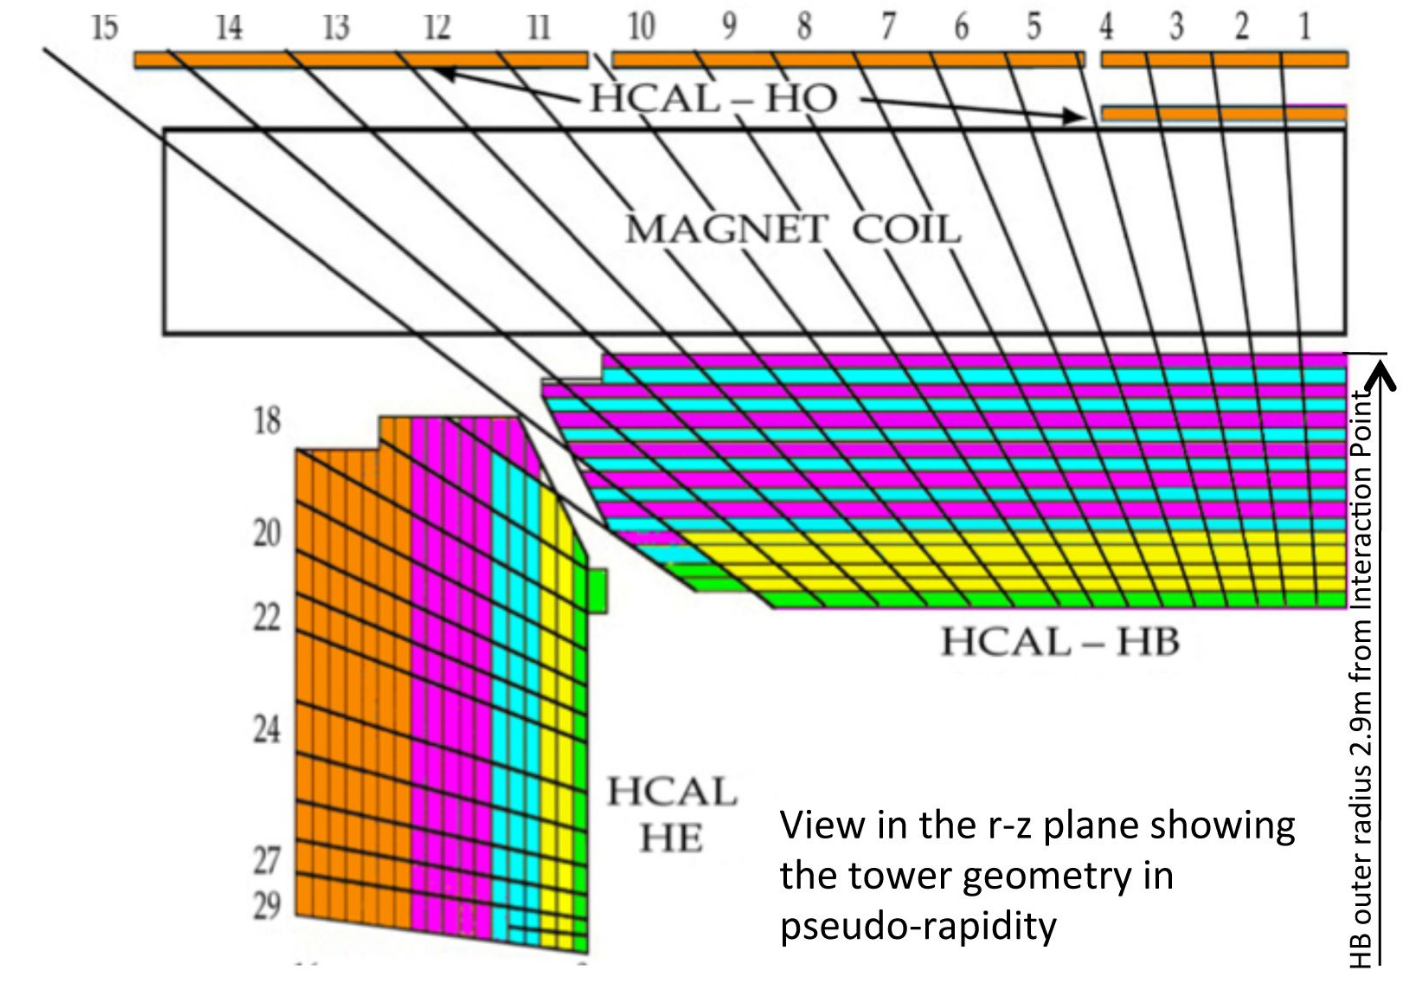
\includegraphics[width=0.4\textwidth]{figures/HCAL_layout.png}
  \caption{\label{fig:HCAL_layout} Layout of the hadronic calorimeter (HCAL) indicating the configuration of the barrel (HB) and endcap (HE) components as well as the outer HCAL (HO) lining the solenoid.}
\end{figure}

\section{The CMS magnet}

The need to measure high $p_{T}$ muons has driven the requirements on the CMS magnetic field strength. With the goal to accurately determine both momentum and sign of 1TeV muons at $\Delta$p/p $\approx $10\%, a superconducting solenoid with an interior magnetic field strength of 3.8T was chosen as the central design feature of CMS.

The solenoid is located outside the silicon tracker, ECAL, and HCAL systems but inside the muon system. Interspersed with the muon system is the steel return yoke, which contains the field outside the solenoid and provides a 2T field to allow the muon system to measure charged particle momentum. 

To generate the magnetic field, 18,160 amperes are passed through four layers of tightly-wound superconducting Nb-Ti wire, resulting in a stored energy of 2.3 gigajoules.

The magnetic field generated by the solenoid bends charged particles according to the equation



$$R = \frac{p_{T}}{0.3eB}$$



where R is the radius of curvature (in meters), $p_{T}$ is the transverse momentum (in GeV), $e$ is the electron charge (in Coulombs), and $B$ is the field strength (in Tesla). Thus, the transverse momentum ($p_{T}$) of the charged particle can be measured from the known field strength and the observed radius of curvature of the tracks measured in the tracker and muon systems.

An artist's rendition of the superconducting solenoid can be seen in Figure~\ref{fig:Solenoid}.

\begin{figure}\centering
  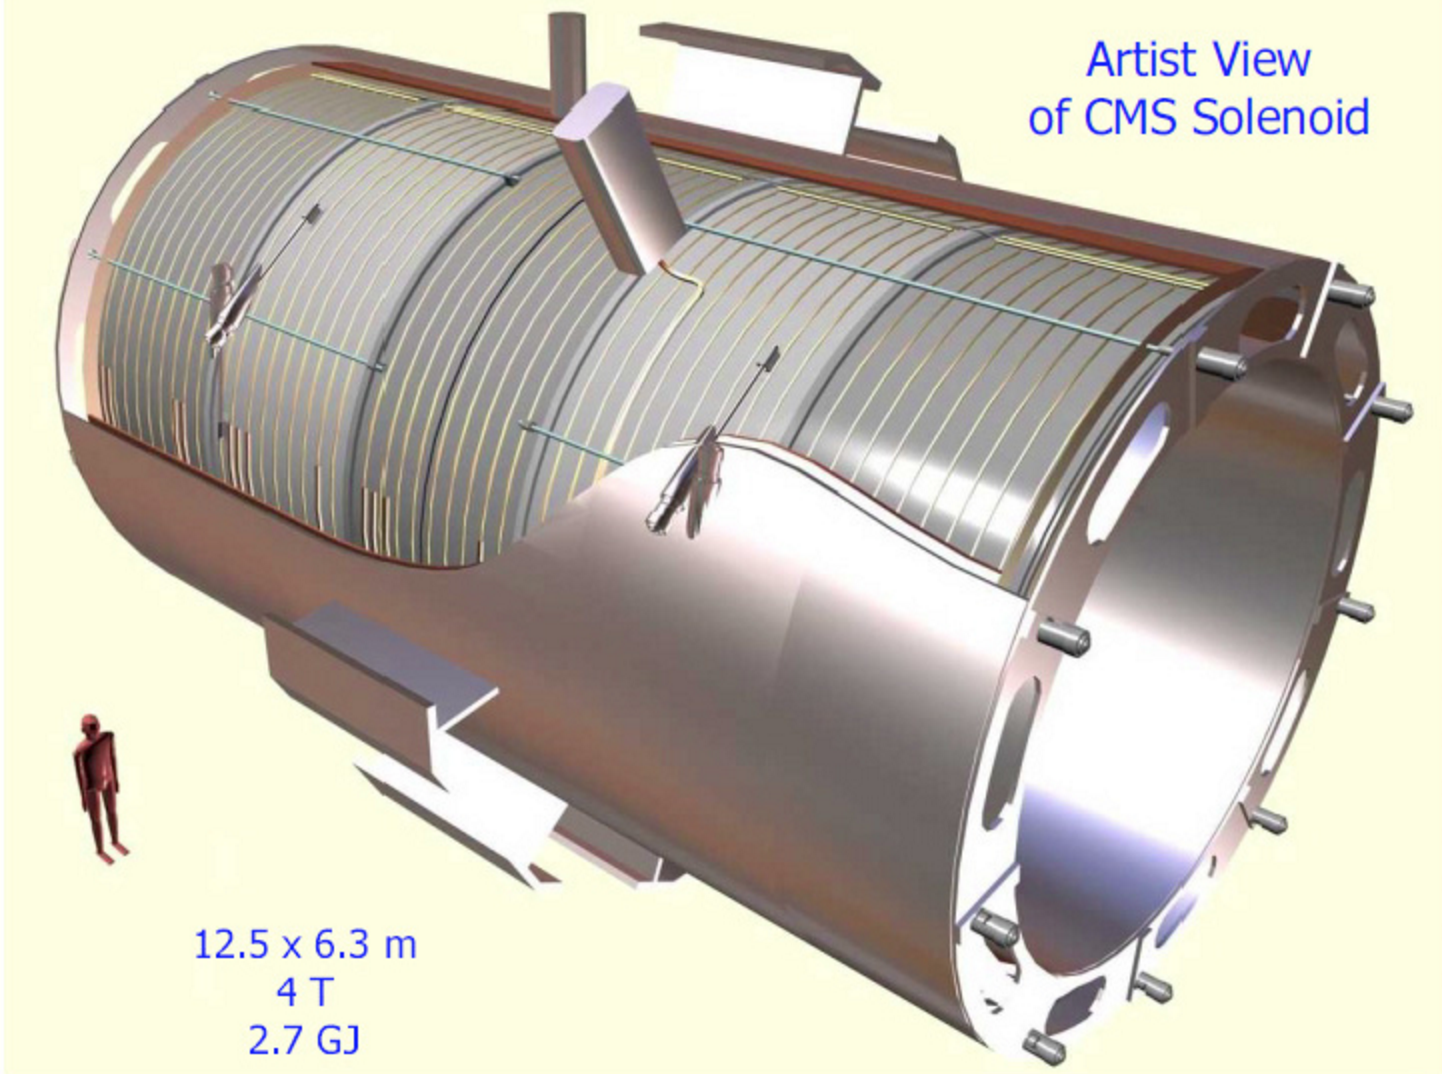
\includegraphics[width=0.4\textwidth]{figures/Solenoid.png}
  \caption{\label{fig:Solenoid} The superconducting solenoid.}
\end{figure}

\section{The muon system}

The muon system is the outermost subdetector, and is central to the design of CMS. It is composed of three separate sensor elements: drift tubes (DTs), cathode strip chambers (CSCs), and resistive plate chambers (RPCs). A diagram of one quadrant of the muon system can be seen in Figure ~fig(muonSystemLayout). "MB" indicates the muon barrel subdetector, which is composed of DTs, "RB" indicates the RPC barrel subdetector, "ME" indicates the muon endcap subdetector (CSCs), and "RE" indicates the RPC endcap subdetector. 

An overview of the layout of the muon system can be seen in Figure~\ref{fig:muonSystemLayout}

\begin{figure}\centering
  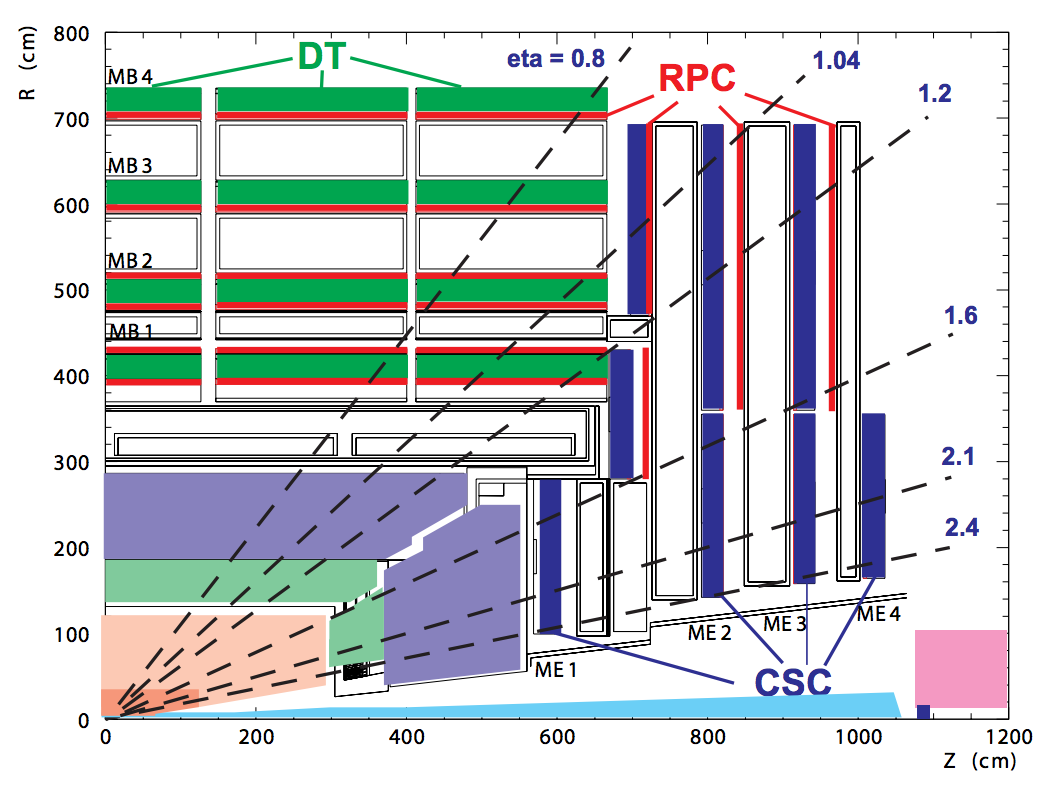
\includegraphics[width=0.4\textwidth]{figures/muonSystemLayout.png}
  \caption{\label{fig:muonSystemLayout} Layout of the muon system highlighting the layered structure of the drift tubes (DTs, green), cathode strip chambers (CSCs, blue), and resistive plate chambers (RPCs, red).}
\end{figure}

\subsection{Drift tubes (DTs)}

The barrel of the muon system contains 250 layers of DTs arranged in four layers (labeled MB1, MB2, MB3, and MB4 in Figure ~fig(muonSystemLayout)). In the MB1, MB2, and MB3 layers, DTs are arranged in 8 $r-\phi$-measuring planes, and 4 $z$-measuring planes. The MB4 layer only contains $r-\phi$-measuring planes.

Each DT is filled with a gaseous mixture of Argon (~85\%) and carbon dioxide (~15\%). Charged particles passing through the DT will ionize the gaseous mixture and produce a current along a central filament to be read out. The maximum drift length per DT is 2.0cm and the single point resolution is $\approx$ 200 $\mu$m.

\subsection{Cathode strip chambers (CSCs)}

The muon endcap (ME) system is comprised of 234 CSCs in each endcap. The CSCs are trapezoidal in shape and are arranged in four layers  (labeled ME1, ME2, ME3, and ME4 in Figure ~fig(muonSystemLayout)). The innermost layer (ME1), is made of 108 CSCs arranged in three rings of 36 CSCs each. The other layers each have two rings (18 CSCs on the inner ring, 36 on the outer ring, for a total of 54 CSCs per layer).

Each CSC is comprised of six gas gaps, with each gap containing a radial array of cathode strips and a plane of anode wires running perpendicular to the cathodes. The CSCs are overlapped in $\phi$ to avoid gaps in the particle acceptance. When a charged particle ionizes the gas, it leaves a charge on the anode wire and an image charge on a group of cathode strips. The spatial resolution provided from each CSC is $\approx$ 200$\mu$m.

The forward (endcap) region of the muon system can expect a higher muon flux, so CSCs were chosen due to their fast response time and fine resolution.

\subsection{Resistive plate chambers (RPCs)}

RPCs can be found in both the barrel and encaps of the muon system, and are used in parallel with the other two subsystems. The RPCs have timing resolution on the order of nanoseconds and are used primarily to resolve ambiguities in cases of multiple hits in the DTs or CSCs, thereby improving the overall accuracy of particle reconstruction.

There are two layers of RPCs "sandwiching" each of the first two DT layers (MB1 and MB2), while the outer DT layers (MB3 and MB4) are paired with one RPC each. The endcap CSCs are also paired with one RPC each. 

Each RPC is comprised of parallel plates of bakelite enclosing two millimeter-thick gas gaps. Each gas gap contains a mixture of 96.2\% R134a (C$_2$H$_2$F$_4$), 3.5\% isobutane (C$_4$H$_10$), and 0.3\% sulfur hexaflouride (SF$_6$).

\section{The trigger system}

When running at full luminosity, the LHC generates $pp$ collisions at a rate of 40MHz. With each event requiring $\approx$ 10MB of digital storage space, this equates to a data-generation rate of 400TB per second. Since this is obviously unsustainable with current computer storage technology, CMS employs a trigger system to reduce the rate of stored events. Two levels of triggering are used: the hardware-based Level-1 (L1) trigger, which reduces the rate from 40MHz to approximately 100kHz, and the hardware-and-software-based High Level Trigger (HLT), which reduces the rate from $\approx$100kHz to 300Hz.

\subsection{The Level-1 (L1) trigger)}

The L1 trigger takes data from the muon system, HCAL, and ECAL in order to make a rapid decision about whether or not to keep the event and send it to the HLT for further review. The L1 triggering rate is about 3.2$\mu$s, during which time the entirety of the data from the event is temporarily stored. Information from the silicon tracker is not used in this stage of triggering, as the time required by the tracker to reconstruct a track is outside this triggering time window. 

The L1 trigger is divided into three major components: the calorimeter trigger, the muon trigger, and the global trigger. The calorimeter trigger looks at the combined (summed) energy deposits in ECAL and HCAL. If the sum is greater than a given threshold, an "accept" signal is sent to the global trigger. The muon trigger looks at the DTs, CSCs, and RPCs which in conjunction form the muon system. If they in concert report at least four muons, each having high transverse momentum and high-resolution tracks ("good"-quality muons), an "accept" signal is sent to the global trigger. The global trigger makes the final decision to reject the event or, if it has received "accept" signals from both the calorimeter trigger and muon trigger, to send it to the HLT.

\subsection{The High level trigger (HLT)}

The HLT is software-based and uses software-defined "HLT paths" in order to determine whether or not a given event will pass a particular physics object selection determined by the path. The advantage of this setup is that different HLT paths can be used by different analysis groups looking for different physics signatures.

The HLT first reconstructs the entirety of the event from the stored data passed to it by the L1 trigger, and determines whether the event passes a given trigger path. There are four broad categories of HLT path: electrons/photons and muons, jets, missing transverse energy ($\MET$), and taus. Hundreds of specific paths offering high levels of discrimination between required selection criteria are available and grouped into these four categories. As the paths are software-based and not hardware-based, new paths can be customized to the needs of any analysis effort.

In order to determine whether or not an event passes a given path, the entire event is reconstructed and run through three broad triggering steps: Stage 2 (calorimetry), Stage 2.5 (calorimetry+pixel hits), and Stage 3 (full reconstruction). In Stage 2, a threshold on calorimeter energy is applied. An object must have a combined ECAL+HCAL calorimetry energy greater than the threshold specified by the path in order to move on to Stage 2.5. In Stage 2.5, information from the pixel subdetector in the silicon tracker is used in order to verify that the hits recorded in the calorimetry towers have corresponding tracks in the pixel system (assuming the particle in question is charged). Finally, in Stage 3, information from the entire detector is used to reconstruct the entirety of objects in the event and ensure that they pass momentum, energy, and quality criteria specified by the path. 



\section{Particle Reconstruction}

Even after a given event has passed the L1 trigger and HLT requirements, its constituent particles only exist as hit patterns in the various subdetectors of CMS. In order for any kind of meaningful physics analysis to be performed, these hit patterns must be turned into physics objects which are more easily-read by the CMS software framework (CMSSW). Broadly, the six principle objects that are "reconstructed" from raw detector data in this manner are: electrons, muons, taus, photons, jets, and missing energy ($\MET$). The chief set of software tools used to reconstruct physics objects is a group of algorithms collectively referred to as Particle Flow (PF).

\subsection{Particle Flow}

Particle Flow (PF) is the term used to refer to the general set of algorithms used to reconstruct physics objects (particles) out of raw detector data. The fundamental inputs to the PF algorithms are the charged particle tracks (from the silicon tracker), hits in the calorimetry towers (from ECAL and HCAL), and hits in the muon system. These fundamental inputs are then grouped into ``blocks" which the PF algorithm translates into physics objects. Muons are identified by matching a track in the tracker with a hit in the muon system, charged hadrons are identified by matching a track in the tracker with a hit in HCAL, and electrons are identified by matching a track in the tracker with a hit in ECAL. Photons and neutral hadrons leave no tracks, so they are identified as hits in ECAL and HCAL, respectively, with no matching tracks. As tracks are matched with calorimetry towers and muon hits, those hits are removed from consideration and whichever tower hits are leftover are assumed to be from photons or neutral hadrons. Once all the visible particles are reconstructed, conservation of momentum principles are applied to infer the missing energy, or $\MET$.

The following subsections will detail the methods used to reconstruct each class of particle, and a final subsection will detail the means by which the event data produced by Particle Flow is packaged into formats useful for analysis efforts.

\subsubsection{Track reconstruction and vertexing}

The goal of the silicon tracker is to reconstruct tracks indicating the trajectories of charged particles through the magnetic field, and furthermore to use these trajectories to ``trace back" the origin of the particle, known as the vertex. The first vertex in each event, that corresponding to the $pp$ collision, is known as the primary vertex (PV). The presence of multiple proton-proton collisions in each bunch crossing, a phenomenon known as pileup, presents the possibility of misidentifying the correct PV for a given event. Therefore, there is a need for a vertexing and tracking algorithms exhibiting a high degree of granularity.

To ensure this, tracks with the highest number of hits in the pixel and strip subsystems within the silicon tracker are recorded (and reconstructed) first. Tracks with three hits, high $p_{T}$, and close proximity to the beam spot are considered to be high quality. These tracks are reconstructed first, and their hits removed. For the remaining, lesser-quality tracks, looser criteria are applied iteratively until all tracker hits have been accounted for.

In order to determine the location of the PV, the reconstructed tracks are clustered together and the location is extrapolated by requiring that each track cluster share a plane compatible with the beam line. This is done online as well as offline so that the PV information can be relayed to the HLT for use in the triggering process. The reconstruction algorithm   uses only information from the pixel subdetector for the online reconstruction, while the offline reconstruction uses information from the entire tracker.

\subsubsection{Electron reconstruction}

Electrons are reconstructed via the combination of a track in the silicon tracker and hits in the ECAL towers. These tower hits are called ``superclusters" and their size in $\eta$ and $\phi$ is dictated by various clustering algorithms selected according to the relevant HLT path. As the electron interacts with the silicon in the tracker, it radiates photons via Bremsstrahlung. This emission causes the electron to bend further in the magnetic field. To account for this, the supercluster size is tuned to catch these Bremsstrahlung photons as well, thereby capturing the total energy of the electron before bending and leading to a more accurate calculation of the electron's energy and momentum. 

To fully reconstruct an electron track, one starts with a track \emph{seed}, which is a possible electron trajectory found by interpolating between layer hits in the pixel and strip detectors. These track seeds must be cleaned and filtered in order to find the most likely track candidate, and then they must be matched with a supercluster in ECAL. There are two methods to achieve this. The first, ECAL driven seeding, begins by reconstructing superclusters in ECAL and attempts to match them with track seeds in the innermost layer of the pixel detector. The track is then reconstructed from these track seeds. The second, tracker driven seeding, begins with a high-quality track seed and attempts to match it to an appropriate supercluster in ECAL, while also taking into account other clusters arising from Bremsstrahlung photons. This is achieved by drawing straight lines tangent to the track towards the ECAL. If a corresponding cluster is found, it is added to the total energy of the electron.

\subsubsection{Muon reconstruction}

Muons can be measured both in the silicon tracker and the muon system. In order to reconstruct a muon, hits in the muon system (\emph{stand-alone muons}) are matched to hits in the tracker in order to reconstruct a complete muon object, known as a \emph{global muon}. These muons are reconstructed using two different methods, \emph{global muon reconstruction (outside-in)} and \emph{tracker muon reconstruction (inside-out)}.

Global muon reconstruction begins in the muon system. Hits in the DTs and CSCs are allocated into segments, which are short stubs containing just enough hits to assign each a momentum and direction vector. These segments are grouped together to form tracks in the muon system. These tracks, known as stand-alone muon tracks, are matched, one by one, with tracks from the tracker by comparing parameters of the two tracks propagated onto a common surface.

Tracker muon reconstruction begins in the silicon tracker. All tracks with $p_{T} > 0.5$ GeV/c and $p > 2.5$ GeV/c are considered possible muon candidates and are propagated outward toward the muon system, taking into account the magnetic field, expected energy loss, and the possibility for multiple Coulomb scattering in the detector material. If a hit in the muon system is found within 3 cm in local $x, y$ coordinates, the candidate qualifies as a tracker muon.

Tracker muon reconstruction is more efficient than global muon reconstruction at low energies ($p < 5$ GeV/c), since it only requires one muon segment in the muon system. Global muon reconstruction is more appropriate for muons with higher energies penetrating through more than one station in the muon system.


\subsubsection{Photon and Neutral Hadron Reconstruction}

Since photons and neutral hadrons are chargeless, and therefore leave no hits in the silicon tracker, the entirety of their reconstruction takes place in ECAL (photons) and HCAL (hadrons). The identification of photons and neutral hadrons takes place via so-called \emph{clustering algorithms} which are designed to separate photons from neutral as well as charged hadrons, and to differentiate photons originating from the primary or secondary decays from those generated by electrons undergoing Bremsstrahlung within ECAL.

Clustering algorithms involve three steps. First, a seed cluster is identified in one of the ECAL towers as a tower with a local energy maximum passing a threshold specified by the algorithm. Next, topological clusters are defined as clusters adjacent to (sharing at least one side in common with) the seed cluster and with cell energies passing another threshold. These thresholds are generally set to be two standard deviations above the base electronics noise level in each of the separate ECAL segments (80MeV in the barrel and 300MeV in the endcaps). Finally, topological clusters then generate as many ``particle flow" clusters as there are seed clusters, and the energy in each particle flow cluster is allocated according to its distance from the seed. 

Furthermore, in particle flow, ECAL/HCAL clusters are required \emph{not} to match any tracks in the tracker in order to qualify as photon or neutral hadron candidates.


\subsubsection{Jet Reconstruction}

Jets are primarily reconstructed in ECAL and HCAL, although their charged constituents usually leave tracks in the silicon tracker as well. The majority of reconstructed jet energy comes from charged particles such as pions and kaons, and a smaller but still sizable portion comes from photons from $\pi^0$ decays in ECAL. Though numerous jet reconstruction algorithms exist, most jet candidates are reconstructed using the Particle Flow (PF) algorithm. The PF algorithm looks at the constituent particles in the jet: charged hadrons, neutral hadrons, and photons individually and then clusters them into jet candidates according to various clustering algorithms, the most common of which is the \emph{anti-}$k_{T}$ algorithm with a cone radius of $R = 0.5$. The energy of photons is determined from ECAL measurements, that of charged hadrons is measured with a combination of tracker, ECAL, and HCAL measurements, and the energy of neutral hadrons is measured according to the description in the previous section.

Approximately 90\% of the reconstructed jet energy comes from charged hadrons and photons, while the remaining 10\% comes from neutral hadrons. Since tracking information from the charged hadrons is available, improved jet vertexing can be done and the impact of pileup can be mitigated.




